\section{Decreasing quote retrieval time}\label{sec:qs}
The legacy quote server can delay for up to four seconds before sending a response.
This delay is vastly greater than the typical command execution time of dozens of microseconds (see~\ref{sec:cmd-dist}).
The legacy server is the greatest barrier to high command throughput and dozens of hours of research and design was spent mitigating the effects of its delay.

\subsection{Statistical analysis of legacy quote server}
We sent a large number of serial requests to the quote server and recorded the response time with a shell script.
Figure~\ref{fig:legacy-qs-hist} shows the distribution of response times follow an exponential distribution with $65.75\%$ of responses experiencing only network delay.
The expected value of the response time is \SI{563.3}{\milli\second}.

\begin{figure}[tbph]
  \centering
  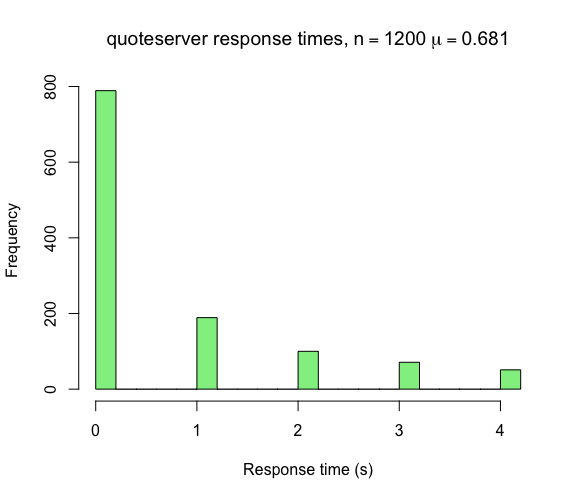
\includegraphics[width=0.6\linewidth]{../../data/quoteserver-times/hist}
  \caption[Legacy quote server response times]{Histogram of legacy quote server response times with \SI{1}{\second} buckets}
  \label{fig:legacy-qs-hist}
\end{figure}

The one second buckets in~\ref{fig:legacy-qs-hist} obscures the fact that results are clustered after whole second values.
Removing the constant delay portion from each bucket yields the distribution (Table~\ref{tbl:qs-net-delay}) of variable network and processing delays.

\begin{table}[htpb]
  \centering
  \caption{Legacy quote server network delays}
  \label{tbl:qs-net-delay}
  \begin{tabular}{@{}cccccc@{}}
    \toprule
    Minimum & 1st Quartile & Median & Mean & 3rd Quartile & Maximum \\ 
    \midrule
    \SI{7}{\milli\second} & \SI{9}{\milli\second} & \SI{9}{\milli\second} & \SI{9.414}{\milli\second} & \SI{10}{\milli\second} & \SI{26}{\milli\second} \\ 
    \bottomrule
  \end{tabular}
\end{table}

From this data we can conclude that if the legacy quote server has not sent a response after \SI{30}{\milli\second} then we will wait at least \SI{1}{\second} for a response.

\subsection{Using timeouts to ensure fast quote retrieval}\label{sec:qs-timeout}
We decided to use a request timeout strategy to minimize the total time spent waiting for a quote.
If there was no response from the quote server after a given timeout we cancel the request by closing the socket connection and issue a new request.
We used the tail of the network delay data (i.e.\ ..., 16, 16, 17, 17, 20, \SI{26}{\milli\second}) to set an initial timeout at \SI{20}{\milli\second} and used a \SI{5}{\milli\second} exponential backoff.
This backoff strategy requires six iterations to exceed the expected delay of \SI{563.3}{\milli\second}.
Exceeding \SI{1}{\second} total delay has a likelihood of 0.0299\%.
If the total timeout exceeds \SI{4}{\second} and there is still no response from the quote server then the service is assumed unreachable and the quote manager raises an error.

\subsection{Timeout effectiveness}\label{sec:timeout-effectiveness}
We implemented the timeout strategy in~\ref{sec:qs-timeout} and gathered response time data directly from the quote manager.
Figure~\ref{fig:retries} shows frequency of retry attempts before a quote resolved.
Strangely, the distribution does not match that of Figure~\ref{fig:legacy-qs-hist} and the legacy quote server has an 89.35\% likelihood (instead of 65.75\%) of resolving in under \SI{20}{\milli\second}.
Day Trading Inc.\ has assured us that the behavior of the legacy quote server is stationary so perhaps the change arises from our serial and timeout-retry request methods.

\begin{figure}[tbph]
  \centering
  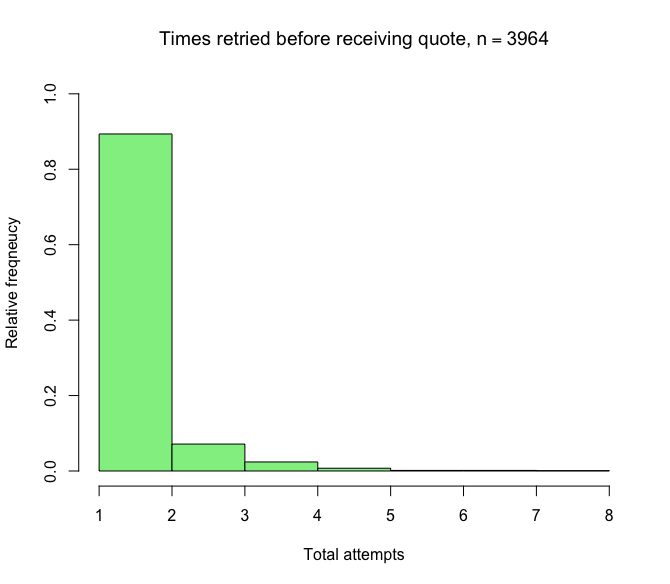
\includegraphics[width=0.6\linewidth]{../../data/quote-times-verification/retries}
  \caption{Quote retry attempt histogram}
  \label{fig:retries}
\end{figure}

The distribution of total waiting times is shown in Figure~\ref{fig:waiting-time}. 89.18\% of quotes are resolved before \SI{50}{\milli\second}.

\begin{figure}[tbph]
  \centering
  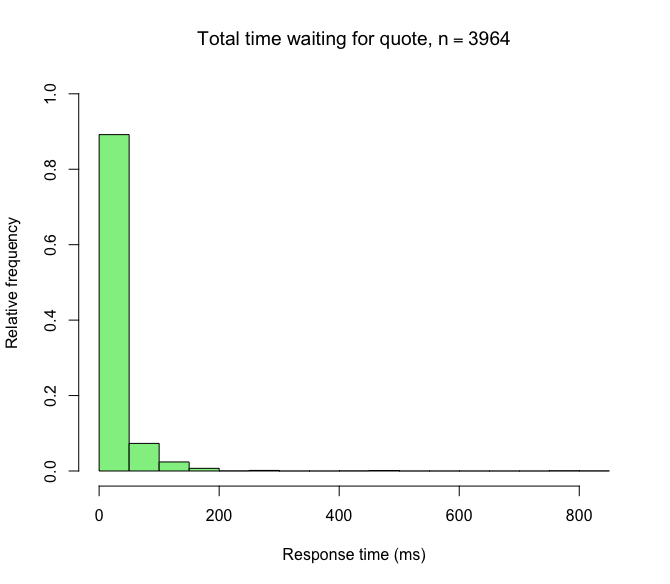
\includegraphics[width=0.6\linewidth]{../../data/quote-times-verification/waiting-time}
  \caption[Total waiting time to retrieve a quote]{Total waiting time to retrieve a quote with \SI{50}{\milli\second} buckets}
  \label{fig:waiting-time}
\end{figure}

Only three quotes take longer than \SI{500}{\milli\second} and none longer than \SI{850}{\milli\second}.
This adds confidence to our derivation that waiting longer than \SI{1}{\second} for a quote should be a $\approx \frac{1}{3400}$ event.

\subsection{Minimizing lingering TCP connections}
When a TCP connection is terminated with a FIN command the socket enters the TIME-WAIT state until the termination is acknowledged with a FIN-ACK command.
The socket stays in the TIME-WAIT state for twice the connection MSL, typically two minutes.
Each open socket occupies approximately 1 Mb of memory and is considered an open file.
Thus, the number of open sockets is limited the the system memory and OS limitation on concurrent open files.

The legacy quote server timeout method necessarily leaves many connections in the TIME-WAIT state.
When we first implemented the timeout method the quote manager would become unresponsive and crash as connections lingered in the TIME-WAIT state and the host had its memory occupied entirely with open TCP connections.

Changing connection methods in our application from the generic \texttt{Dial} method to the specific \texttt{DialTCP} method resolved the lingering connection issue.
We suspect that \texttt{Dial} discards the connection in such a way that the FIN-ACK is not received by the socket and the OS maintains the connection for the entire double MSL period.
This difference is behavior is undocumented and should be disseminated to developers who use Go in applications with high TCP socket turnover.
